\subsubsection{Link between geophysical parameters and mineralogy and temperature}
\label{sec:geo_min_link}

In order to predict the seismic properties of Mars' mantle, equations of state must be formulated that describe the pressure- and temperature-dependence of the bulk modulus, shear modulus and density. The basis for most equations of state is a relationship between pressure and elastic constants at room temperature, for which a variety of high pressure formulations exist \citep[e.g.][]{Stacey2004}. One of the most popular is the Birch-Murnaghan (BM) finite-strain theory \citep{Murnaghan1944,Birch1952}, in which the Eulerian elastic strain energy is expanded as a Taylor series. A third-order expansion is reasonably accurate when pressures are a small fraction of the zero-pressure bulk modulus \citep{Stixrude2005}. Most endmembers of mantle minerals have bulk moduli greater than 100 GPa, and so a third-order BM expansion is reasonable up to 25 GPa, covering the entire pressure range of Mars mantle.

There are several different approximations which have been used to extend room temperature equations of state to high temperature $T$. \cite{Anderson1988} and \cite{Duffy1989} advocate extrapolating standard state properties to high temperature at 1 bar by fitting volume data to a thermal expansion model based on Gr\"uneisen theory, and making the assumptions that $\{M\}_P$ is constant and \{$\partial$$M$/$\partial$$P$\} = -1 (where $P$ is the pressure, \{[$\cdot$]\}=$\partial$$ln$[$\cdot$]/$\partial$$ln$$\rho$, and $M$ is either the isentropic incompressibility $K_S$ or shear modulus $\mu$). The resulting values of $\rho$, $K_S$ and $\partial$$K_S$/$\partial$$P$ are then substituted into the BM finite strain expressions to extrapolate to high pressure along an adiabat. This formulation has been used in studies of Mars by \cite{Mocquet1996}, \cite{Verhoeven2005}, and \cite{Rivoldini2011}. Using a slightly different approach, \cite{Bina&Helffrich1992} fitted 1 bar volume data to a polynomial, approximated $\{K_T\}_P$, $\partial$$\mu$/$\partial$$T$ and $\partial$$K_T$/$\partial$$P$ as constant at 1 bar, and then extrapolated to high pressure along an isotherm, again using the BM finite strain expressions. Finally, they derived $K_S$ from $K_T$ using Gr\"uneisen theory. This formulation has been used in studies of Mars by \cite{Sohl1997}, \cite{Bertka1998}, and \cite{Zharkov2005}.

While the above formulations allow the direct use of abundant 1 bar thermal expansion data \citep[e.g.][]{Saxena1992}, there are problems with equations of state that rely on integrating along 1 bar paths. Firstly, at low pressure, anharmonicity can contribute significantly to material properties, and many minerals become unstable before reaching mantle potential temperatures, such that extrapolations to high temperature are required. Secondly, the use of the BM expansions to calculate the elastic moduli at high pressure implicitly constrains other thermodynamic properties such as the heat capacity through Maxwell relations \citep[e.g.][]{Fegley2013}, but does not impose reasonable constraints on the functional forms of these properties. As a result, it is possible for equations of state to return unphysical properties, especially at high temperature. In the pressure-temperature range of Mars' mantle, the associated errors are usually small, but an improved approach is still warranted.

An alternative to the isobaric approaches above is to instead define a thermal equation of state based on isochoric (constant volume) extrapolations, in which high temperature properties are derived via a thermal pressure term. This term is typically derived from theoretical models of phonon contributions to the thermal energy, such as Debye or Einstein models \citep{Stixrude2005,Matas2007,Holland2011}, along with a description of the volume dependence of the thermal energy via a functional form for the Gr\"uneisen parameter. Such formulations have a more robust physical grounding, and therefore typically provide estimates of physical properties which are in better agreement with raw ab-initio calculations and shock experiments (Thompson, 1990). 

Once equations of state have been defined for the appropriate mineral end-members, it is necessary to describe how the physical properties of mantle minerals vary when they contain components of more than one end-member. For example, olivine in Mars mantle is believed to contain significant forsteritic (\ce{Mg2SiO4}) and fayalitic (\ce{Fe2SiO4}) components. Following the results of high pressure experiments performed at the laboratory, some studies make the assumption that density, bulk and shear modulus are linear functions of the iron content at standard state conditions \citep{Mocquet1996,Verhoeven2005,Rivoldini2011}. \cite{Khan2008} and \cite{Khan2018} instead used the ideal solution model approximation where the volume of the mineral is equal to the molar-weighted arithmetic average of the end-member volumes at constant pressure and temperature, and the bulk and shear moduli are the volume-weighted harmonic average at constant pressure and temperature \citep{Stixrude2005}. The ideal solution model is more easily incorporated into Gibbs minimization routines (see below), allowing for a self-consistent equilibrium description of Mars mantle. However, there is otherwise little practical difference between the choices, as the major end-members within mantle solid solutions tend to have quite similar properties (with a few notable exceptions, such as pyrope-grossular garnets).

Finally, the properties of each mineral are averaged to obtain an estimate of bulk properties. Voigt-Reuss-Hill \cite{Hill1952} averages usually produce reasonable estimates of seismic properties within untextured rocks, and \cite{Hashin&Shtrikman1963} bounds provide a useful range within which effective isotropic velocities should lie.

In most of the previously mentioned studies \citep{Mocquet1996, Sohl1997, Bertka1998, Zharkov2005, Verhoeven2005, Rivoldini2011}, the computations of the mineralogical composition of the mantle, and of its seismic properties, are performed separately. The mineralogical composition is generally computed from chemical oxide compositions derived from geochemical studies \citep[reviewed in, e.g.][]{McSween1994, Taylor2013}, possibly constrained by laboratory synthetic experiments \citep{Bertka1997}, at the pressure and temperature conditions that are subsequently used to compute the seismic parameters. In this approach, phase equilibria and physical properties are thus generally not mutually consistent from a thermodynamic point of view.

A self-consistent description of both mineralogical phase equilibria and physical properties is achieved by minimizing the Gibbs free energy subject to fixed bulk composition constraints (Connolly and Kerrick, 2002; Connolly, 2005; Stixrude and Lithgow-Bertelloni, 2005b, 2011). This technique was used by \cite{Khan2008} and \cite{Khan2018} to model Mars interior, and will be followed to invert for interior structure during the InSight Mission.

\subsubsection{Comparison and benchmark of the InSight Geophysics Mineralogical mappers}
%(Verhoeven, Khan, Rivoldini, Gudkova, Mocquet, Myhill)
%\textcolor{orange}{[50 lines for this sub-section, describing the softwares validated in the benchmark exercise. Details of each approach will be summarized and mostly linked to references. Descriptions of the models used for benchmark (e.g. mineralogy and temp??rature, table or figure) and results of the benchmark (vp, vs, rho, other benchmarked parameters). Total 1.5 page]}

Synthetic density, $\rho$, and seismic velocities $V_P$ and $V_S$ are computed for a given model of temperature and composition in Mars' mantle using the code Perple\_X \citep{Connolly2009} developed by James Connolly (http://www.perplex.ethz.ch) and used by \cite{Khan2018} to invert Martian geophysical data such as mean mass, moment of inertia and tidal response.

This method relies on Gibbs free-energy minimization to compute stable mantle mineralogy and physical properties along self-consistent mantle adiabats and uses the thermodynamic formulation of \cite{Stixrude2005} and parameters of \cite{Stixrude&Lithgow-Bertelloni2011} within the chemical system \ce{Na2O-CaO-FeO-MgO-Al2O3-SiO2} (NCFMAS).

A range of different compositions are chosen to sample the whole set of published models of the Martian internal structure \citep[see][]{Panning2016} and are associated with hot and cold end member temperature profiles computed from thermal evolution models \citep{Plesa2016}. An alternative to Perple\_X to compute density and seismic velocities at Martian conditions is to use a parameterized phase diagram approach along with experimentally derived thermodynamic and elastic parameters. Such an approach was used by \cite{Vacher1998} to highlight the role of the non-olivine components in the 660 km depth discontinuity in Earth mantle. The two methods have different strengths and weaknesses. The Gibbs minimization technique computes a thermodynamically self-consistent equilibrium planet, and therefore relies on accurate thermodynamic parameters, both for the endmember phases and for the solid solutions. The \cite{Vacher1998} algorithm is generally thermodynamically inconsistent, but provides additional flexibility to investigate non-equilibrium scenarios or the effects of chemical changes within individual mineral phases.

Figures \ref{fig:FigDWTh.png} and \ref{fig:FigDWThdiff.png} show a comparison between the outputs produced by the two methods for the Dreibus-W\"{a}nke composition \citep{Dreibus&Wanke1985} and the hot end-member temperature profile of \cite{Plesa2016}. As can be observed in Figure \ref{fig:FigDWThdiff.png}, spikes are present in both density and seismic wavespeed differences and correspond to small differences in the location of phase transitions estimated by the two codes. Aside from these spikes, though, the difference in density values computed with the two codes is less than 50 kg/m$^3$ and the wavespeed difference is less than 0.2 km/s. The origin of these differences is twofold. The first one is related to differences between the mineralogy computed by Perple\_X from NCFMAS oxide composition and the mineralogy from literature values used in the parameterized phase diagram approach. The second one is related to the values of the elastic and thermodynamic parameters used to extrapolate density and seismic wavespeeds from reference conditions to pressure and temperature conditions of the Martian mantle.

\begin{figure}[h!]
\begin{center}
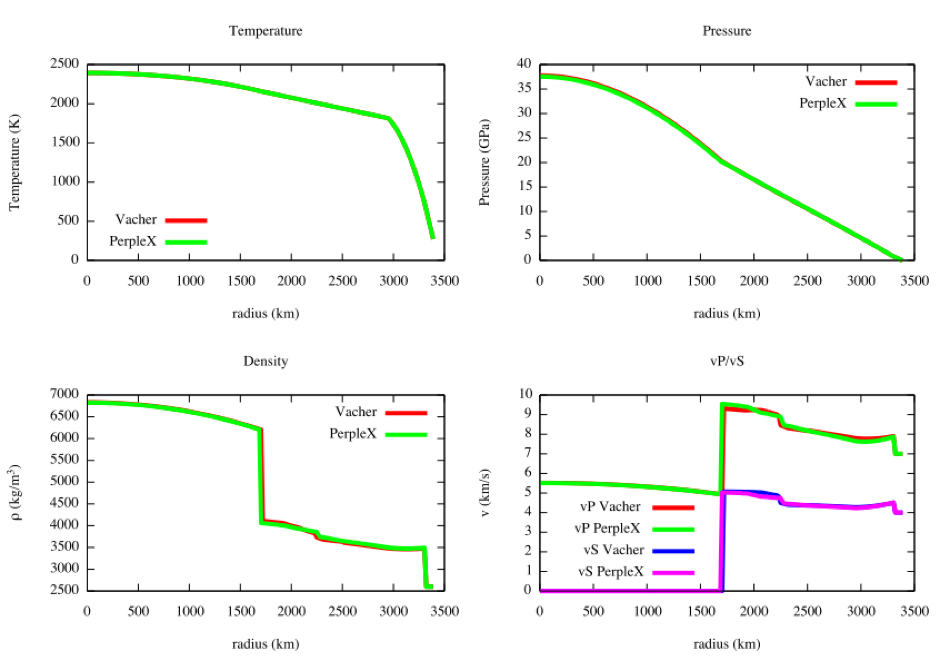
\includegraphics[width=0.85\textwidth]
{figures/FigDWTh.png}
\caption{Temperature, pressure, density and seismic velocities profiles in the Martian mantle for a Dreibus-W\"{a}nke composition \citep{Dreibus&Wanke1985} associated to the hot end-member temperature profile of \cite{Plesa2016} and computed with the two Geophysics Mineralogical codes (Vacher for \cite{Vacher1998} and Perple\_X for \cite{Connolly2005}).}
\label{fig:FigDWTh.png} 
\end{center}
\end{figure}

\begin{figure}[h!]
\begin{center}
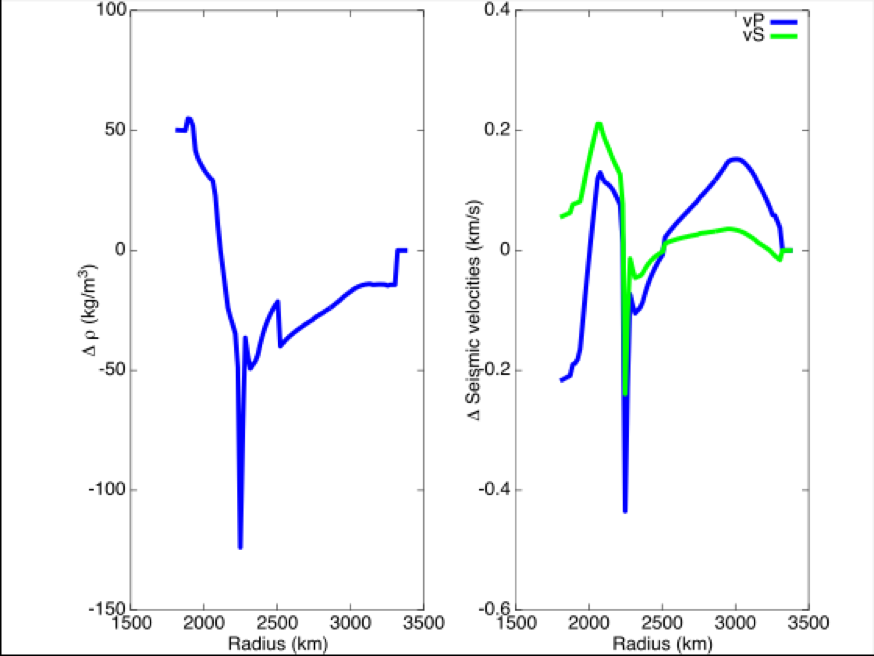
\includegraphics[width=0.65\textwidth]
{figures/FigDWThdiff.png}
\caption{Difference in density and seismic velocities values computed with the two Geophysics Mineralogical codes for a Dreibus-W\"{a}nke composition (Dreibus and W\"{a}nke, 1985) associated to the hot end-member temperature profile of Plesa et al (2016). The location of the phase transition at radius of approximately 2300 km differs by about 30 km between the two codes, leading to a large peak at that depth.}
\label{fig:FigDWThdiff.png} 
\end{center}
\end{figure}

\subsubsection{Discussion of the uncertainties of mineralogical modeling}
\label{discussionofuncertainties}
%\textcolor{orange}{(Rivoldini, Myhill, Verhoeven, Khan, Gudkova)
%thermodynamic equilibrium and introduction of oxygen and sulfur as independent components to the mantle.
%[30 lines. What is missing from the approach of the above section, estimations of the uncertainties. Maybe one Figure, but error bars will be added to the figures of 3.2.1.2 and of 3.3. Total 1 page]}

%In this subsection, we discuss the sources of uncertainty associated with forward modelling seismic velocities in Mars??? mantle. We will limit this discussion to uncertainties associated with modelling a homogeneous, texturally isotropic mantle in local thermodynamic equilibrium
While there are many possible sources of error associated with forward modeling of seismic velocities in Mars' mantle, we first consider here the uncertainties associated with modelling a homogeneous, texturally isotropic mantle in local thermodynamic equilibrium.
In the infinite-frequency limit and for a rock of a given composition at a given pressure and temperature, errors in modelled seismic velocities can arise from two sources: 1) inability of the equation of state, solution model and aggregate formulations to match real behaviour, and 2) incorrect thermodynamic and elastic parameter values for the endmember or solution models. 

For the majority of silicate and oxide minerals relevant to Mars' mantle, the quasiharmonic approximation of Stixrude and Lithgow-Bertelloni (2005; 2011) provides a reasonable estimate of elastic seismic velocities. Jacobs et al. (2017) show that thermodynamic models described using a single (volume-dependent) Einstein or Debye temperature can produce seismic wave velocities within 1\% of the measured velocities over a range of pressures and temperatures spanning much of Earth's upper mantle. 

The largest contributor to errors in seismic velocity calculations is probably uncertainty in laboratory measurements. Both the location of phase transitions and the seismic velocities of phases at high temperature and pressure can differ significantly between studies. For example, the pressure of the ringwoodite to bridgmanite + ferropericlase reaction varies by $\sim$2 GPa between different research groups (c.f. Ye et al., 2014). As another example, the aggregate $V_P$ and $V_S$ velocities of San Carlos olivine (fo90) derived from Brillouin spectroscopy can differ by as much as 2\% at high pressure (Zha et al., 1998; Mao et al., 2015), for reasons that are not yet clearly understood, but may be the result of nonhydrostatic stresses in the diamond anvil cell. Connolly and Khan (2016) recently made the first effort to quantify the seismic implications of experimental uncertainties. 

Aside from any updates and extensions to existing datasets, mineralogical mapping for the InSight Mission will be conducted with the thermodynamic dataset of Stixrude and Lithgow-Bertelloni (2011). This dataset contains minerals in the chemical system \ce{Na2O-CaO-FeO-MgO-Al$_2$O$_3$-SiO$_2$}. This system probably accounts for $>$97 wt\% of the bulk composition of Mars (Dreibus and W\"{a}nke, 1984), and therefore any additional components will have a small influence (probably <10 m/s) on seismic velocities. Nevertheless, it is worthwhile to consider the hosts for minor components in Mars' mantle. The most significant of these are probably MnO, Cr$_2$O$_3$ and S, which are all predicted to have abundances of $>$0.2 wt\% in Mars (Dreibus and W\"{a}nke, 1985; Tuff et al., 2013). At low oxygen fugacity, sulphur in Mars' mantle will be incorporated into iron sulfide. Manganese readily substitutes for magnesium or iron within olivine, pyroxene and garnet (Nishizawa et al., 1972; Balta et al., 2011), and is therefore unlikely to significantly affect phase proportions or stabilities in Mars' mantle. In contrast, chromium is preferentially incorporated into spinel at low pressures, stabilising it relative to other alumina-rich phases such as feldspar and garnet (Ziberna et al., 2013). Although chromium is not included in the Stixrude and Lithgow-Bertelloni dataset, it is included in the NCFMASCrO solution models of Jennings and Holland (2015). Using this dataset with the Dreibus and W\"{a}nke (1985) bulk composition, we investigate the effect of including Cr$_2$O$_3$ rather than replacing it with a mole-equivalent amount of Al$_2$O$_3$. Chromium expands the spinel stability field from a narrow wedge between the plagioclase and garnet-bearing fields restricted to $<$1000 K and $<$0.8 GPa to a field that extends up to the melting point at ~1.5 GPa. Bulk sound velocities increase by 0.2-1\% where spinel partially replaces plagioclase (at $<$1 GPa), and decrease by up to 1\% where spinel partially replaces garnet. The decrease in velocity due to adding chromium persists at higher pressure where spinel is not stable, but the perturbation is reduced to $\sim$0.25\%. This reduction is equivalent to a $\sim$50 K increase in temperature (for Vp $\approx$ 8 km/s and dVp/dT $\approx$ 0.4 m/s/K).

One additional independent component that is not included in the current modeling effort is oxygen. At low pressures, Mars is sufficiently reduced that iron is present almost exclusively as Fe$^{2+}$, either within silicate minerals or iron sulfide. At high pressures, however, iron undergoes an autoredox reaction, producing metallic iron and Fe$^{3+}$ (e.g. Frost and McCammon, 2004; Rohrbach et al., 2007). Although this reaction has not yet been documented in Mars-like compositions, it should take place regardless of the bulk composition. Near to the base of Mars' mantle, the main host for ferric iron is garnet, such that the key reaction will be

\ce{3Fe2SiO4} (ferroringwoodite) $\rightarrow$ \ce{Fe3Fe2Si3O12} (skiagitic garnet) + Fe (metallic iron/sulfide).

This reaction will reduce the amount of ringwoodite relative to calculations assuming all iron as Fe$^{2+}$. According to the model of Jennings and Holland (2015), skiagitic garnet has a bulk sound velocity 94\% that of ringwoodite at the P-T conditions of Mars' deep mantle. Ferric-ferrous iron ratios in majoritic garnets from laboratory experiments suggest that a skiagitic component may be the dominant iron-bearing endmember at $>$14 GPa (Rohrbach et al., 2007). The experiments of Bertka and Fei (1997) suggest that $\sim$40\% of Mars' lowermost mantle is garnet and that a skiagite component comprises $\sim$20\ mol \% of this garnet. In this case, one should expect a 0.5\% velocity reduction due to the autoredox reaction. Work is in progress to better understand the chemical and physical implications of these reactions on Mars' deep mantle.

\subsubsection{Pre-launch review of the geophysical parameters}
\label{sec:geophys}
%Review of the existing models for density, vp, vs, electrical conductivity, Qs, (Panning, Johnson, Khan, Giardini, van Driel, Staehler, Langlais, Gudkova, Mocquet, Dehant) [30 lines, May focus more on the historical evolution of the a priori models, from the mid 70th ( e.g. MARS AR, i.e. a PREM like model only corrected from pressure) to the modern a priori models and those defined as a priori model for InSight. Maybe add the Figure shown by V.Dehant on the Evolution of the core radius in the literature, with the most recent updates. Total 1 page]
\paragraph{Bulk structure constraints}
Prior to good constraints on Mars radius and oblateness from Mariners 4 and 9, the earliest estimates of Mars interior structure varied from estimates with a small dense core (Jeffreys, 1937) to a mostly undifferentiated body (Urey, 1952).  After the Mariner 4 flyby in 1965, and the Mariner 9 orbiter in 1971, improved estimates of the normalized polar moment of inertia (C/MR$^2$, where C is rotational moment of inertia, and M and R are the mass and radius of Mars) to $\sim$0.377, assuming hydrostatic equilibrium, allowed for improved models with either small Fe-Ni cores (Binder, 1969) or a range of larger core sizes with a mixture of Fe and FeS (Anderson, 1972; Johnston et al., 1974).  By the late 1970's, the estimate of the moment of inertia had been further revised to 0.3654 after taking into account isostatic compensation and the mass of Tharsis (Reasenberg, 1977), which is closer to refined estimates after the Pathfinder mission in the 1990's of 0.3662 (Folkner et al., 1997), although a broad range of values from 0.345 to 0.365 was still permitted by the data (e.g. Bills, 1990).  Improved models at this time matched this value and assumed simple layered models (crust, mantle with a phase transition corresponding to the olivine-spinel transition, and core), with linear gradients of elastic and density structure within these layers scaled from Earth models by the lower pressure gradient, e.g. model AR (Anderson et al., 1977; Okal and Anderson, 1978).  There have been many further refinements since this time, taking into account refined estimates of Martian chemical makeup and thermal structure, and improved mineral physics modeling to more accurately represent density, elastic and attenuation structure as discussed in more detail in section \ref{sec:geo_min_link} (Zharkov et al., 1991; Longhi et al., 1992; Kuskov and Panferov, 1993; Mocquet et al., 1996; Sohl and Spohn, 1997; Yoder and Standish, 1997. Bertka and Fei, 1998; Sanloup et al., 1999; Zharkov and Gudkova, 2000, 2005; Kavner et al., 2001; Yoder et al., 2003; Gudkova and Zharkov, 2004; Verhoeven et al., 2005; Sohl et al., 2005; Khan and Connolly, 2008; Zharkov et al., 2009; Rivoldini et al., 2011, Wang et al., 2013; Khan et al., 2017). 

\paragraph{Constraints on the core}
%(Weber, Rivoldini, Giardini, Garcia, Johnson, Dehant)
%[30 lines, focus on the a priori constraints for geophysical parameters (e.g. density, vp, vs if inner core, electrical conductivity, core ellipticity, etc., 2 Figures, Total 1 page]

After the moment of inertia number had finally been constrained after the Mars Pathfinder mission (Folkner et al., 1997), many new models were created using a variety of chemical models for Mars (e.g. Dreibus and W/"{a}nke, 1985; Morgan and Anders, 1979). Further progress can be associated with constraints on the tidal Love number k2 (Yoder et al., 2003), which showed Mars to have a liquid core. While the proposal of a liquid Martian core was made previously (e.g. Lognonne and Mosser, 1993; Zharkov and Gudkova, 1993, 1997), many earlier models had assumed a solid core due to the lack of a significant internal magnetic field.  Further model refinements were permitted by laboratory experiments on the compressibility and phase transformations of the predicted compositions of the Martian mantle using laboratory high-pressure facilities at high temperatures such as those performed by Kamaya et al. (1993) for the chemical model by Morgan and Anders (1979) and for the Dreibus and W\"{a}nke (1985) model by Bertka and Fei (1997, 1998).

Recent models of Mars are qualitatively similar, although modeling methods differ. The current best estimate of the radius of the Martian core ($\sim$1720-1810 km) (Khan et al., 2018) has increased substantially due to the increased value of k2 (Konopliv et al., 2006, 2011, 2016) in comparison with Yoder et al. (2003).  Overall, one of the biggest sources of uncertainty in a priori modeling of Martian structure remains the tradeoff between core density and size (figure \ref{fig:Figsulfur.png}).

\begin{figure}[h!]
\begin{center}
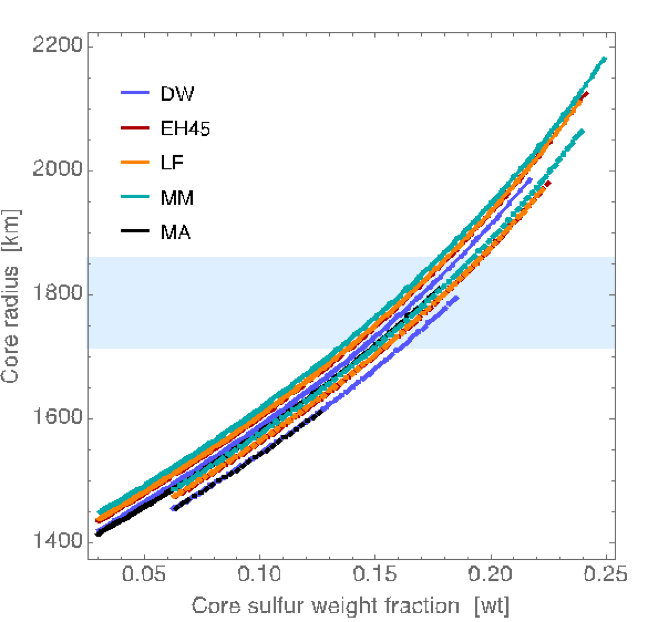
\includegraphics[width=0.65\textwidth]
{figures/Figsulfur.png}
\caption{Core radius as a function core sulfur concentration for the hot (solid curves) and cold (dashed curves) mantle temperature profile.  The blue shaded area represents the core radius range in agreement with the k2 value of Konopliv et al. 2016 and Genova et al. 2016. The acronyms stand for the different mantle mineralogy models (DW: Taylor [2013], EH45: Sanloup et al. [1999], LF: Lodders [2000], MM: Mohapatra and Murty [2003], MA: Morgan and Anders [1979]. Models agree at 1-sigma with the average moment of inertia of Mars (MOI=0.3639$\pm$0.0001) [Konopliv et al., 2016].}
\label{fig:Figsulfur.png} 
\end{center}
\end{figure}
All these models provide relatively large core rich in sulfur, implying that an inner core is quite unlikely today.

%\textcolor{purple}{Notes from Tilio:
%I am not aware of any publication showing vs profiles for the inner core. I have addressed the question of the presence of an inner core in dpi: 10.1016/j.icarus.2011.03.024.
%But in that publication I did not show the vs profiles in the inner core. Needless to say, the large core of Mars requires quite a lot of sulfur implying that an inner core is quite unlikely today.
%Moreover, because of the large amount of S, solid Fe crystallization if the core temperature would allow for it, would result in snow formation, possibly leading to top-down inner core formation if 
%the composition in sulfur is below the eutectic composition and to the formation of Fe-S compounds if the composition of the core is larger than the eutectic composition. Those compounds might sink or float up. But his has not been studied in detail yet. A discussion of this can be found here doi: 10.1186/s40645-017-0139-4. As you can see from that publication, for crystallization to happen at all a very low temperature is required, not at all in agreement with thermal evolution models. If required I can produce figures that show velocities in the core and inner core, but the core radii of those models are small and not in agreement with observed tides.}

\paragraph{Constraints on seismic attenuation}
The first discussion on seismic attenuation in the Martian interior was by Lognonn\'{e} and Mosser (1993) where the authors converted the shear attenuation, Q$_{\mu}$, distribution of the Earth model PREM (Dziewonski and Anderson, 1981) to the conditions of Mars, accounting for temperature differences and integrated from the Q estimated from the Phobos tide secular acceleration. More detailed investigation of anelasticity of the Martian interior and estimates of the dissipative factor were then considered in Zharkov and Gudkova (1997) and more recently by Zharkov et al. (2017). All these first studies were based on the extrapolation of an Anderson and Given (1982) attenuation model to Mars conditions, in which seismic Q is defined as a power law function of frequency with an exponent $\alpha=0.15$ in a seismic bandwidth between corner frequencies $f_1$ and $f_2$ and a steeper exponent of 1 or -1 below or above the bandwidth, respectively. More recently, Khan et al (2016, 2017) proposed to use a consistent model for the frequency dependency of both Q and seismic velocities based on a Burger derived model from the work of Jackson and Faul (2010). This model, however, essentially also predicts effectively a power law for Q (e.g. Bellis and Holtzman, 2014) with a larger exponent $\alpha \approx$ 0.2--0.3 in the seismic bandwidth, but a less steep slope ($1-\alpha$) for frequencies below the seismic band.  Although many experimental data support a relatively constant power law at frequencies less than 0.1 Hz and therefore a Q increase towards high frequencies, experimental data (e.g. Jackson and Faul, 2010, Fontaine et al., 2015) shows that such a constant power above 0.1Hz is not a robust assumption, as the Q might converge towards a plateau around 1 Hz and even decrease at higher frequencies.  In addition, large discrepancies are already found between Earth observations and laboratory data, as summarized by Lekic et al. (2009) and Romanowicz and Mitchell (2007, 2015). Understanding the frequency dependence of Q is essential in order to relate attenuation within the seismic band to constraints at the Phobos tidal period.  Using different estimated exponential slopes for the Q frequency dependence from the estimated Phobos Q (85 $\pm$ 5), which is mostly controlled by average Q$_{\mu}$ in Mars' mantle at tidal frequencies, could lead to Q increase by a factor of 2.1, 3.1 and 4.6 at 10 sec respectively for $\alpha$=0.1, 0.15, 0.2, and therefore to larger Q at 1 Hz. Proposed values range therefore from less than about 200 for Zharkov and Gudkova (2017) and Khan et al. (2018) who use $\alpha\leq 0.1$ to 250-300 for Lognonn\'{e} and Mosser (1993) and Zharkov and Gudkova (1997), who used 0.15.

%Nevertheless and to first order, the Phobos Q = 85 ? 5, as mostly related to the average shear Q in the Mars Mantle, could lead to Q increase by a factor of 2.1, 3.1 and 4.6 at 10 sec respectively for a=0.1, 0.15, 0.2, and therefore to large Q at 1 Hz (ranging from 250 to 300 for Lognonn? & Mosser, 1993, Zharkov and Gudkova, 1997 who used 0.15 but less and about 200 for ?and Zharkov and Gudkova, 2017).

Another approach to estimating seismic Q on Mars rather than the use of the Phobos tide Q might be based on scaling from Earth observations. This is based on the assumption that Q is given by (e.g. Jackson et al., 2002)
\begin{equation}
Q^{-1}=A\left[ { 1 \over f d}\exp\left(-{E+pV \over RT}\right)\right]^{\alpha},
\end{equation}
where $A$ is a constant, $a$ the power law slope, $f$ and $d$ the frequency and grain size, $E$ and $T$ the activation energy and thermodynamical temperature, while $p$ and $R$ are the pressure and ideal gas constant, and $V$ is the activation volume. By taking (2) for a given frequency, pressure and size grain but two different temperatures T and T$_0$, we then get :
%\textcolor{red}{Mark: Please check this equation, which was written as Q-1=A[f-1d-1exp(-E+pVRT)] in the original Word file by Philippe, which was hard to read and appeared to have the wrong frequency dependence. I've attempted to correct it, but I may have introduced new errors.  I also added a $b$ term to the equation below, which was missing from the original Word file but referenced in the following text, and changed it to a $\Delta T$ rather than T, which makes more sense, unless you define $Q_0$ at 0K.  I also called $V$ the activation volume... is this what you meant?} This leads to a temperature dependency of Q which can be written as
\begin{equation}
Q^{-1}(T) = Q_0^{-1}\exp\left(-b \ ({1 \over T} - {1 \over T_0})\right) ,
\end{equation}
where $Q_0$ is the observed quality coefficient at a reference temperature $T_0$ and Q the predicted one at T. Here, $b=\alpha \ {E+pV \over RT}$.
% originally written as Q-1 = Q0-1exp(-T), which didn't exactly make sense
 Large variations remains however in estimation of the $b$ parameter, which range from $\sim$13500 K for Jackson et al (2002) (for E=424kJ/mole, $\alpha$=0.26, p=0) to 3540 K for Fontaine et al. (2005). We use the value of Lognonn\'{e} \& Mosser (1993) of 4530 K as a mid range example (with E=251kJ/mole, $\alpha$=0.15), and extrapolate from the reference Q of 173 for the Earth's upper mantle (outside the Earth Low Velocity zone) based on the PREM model (Dziewonski and Anderson, 1981). This is shown for the difference a priori reference Mars models and associated temperature structures in Figure \ref{fig:FigshearQ.png}. For depth less than 300 km, all Mars models suggest a mantle colder than Earth at the same pressure, and likely larger Q. But deeper than 300 km, the Earth mantle could in contrast be colder than Mars for the same pressure, and temperature effects will reduce Q.

\begin{figure}[h!]
\begin{center}
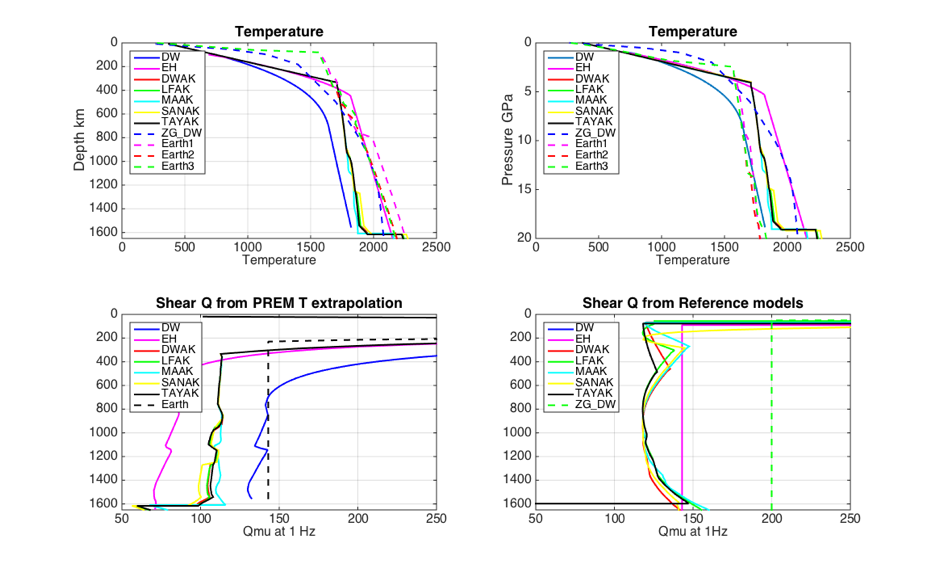
\includegraphics[width=1.1\textwidth]
{figures/FigshearQ.png}
\caption{On the top, Reference models temperature as function of depth (on the left) and Pressure (on the right) as compared to Earth Temperature models. See section 3.3 for more details on these reference models. On the bottom, comparison between on left, the shear Q as extrapolated from PREM with relation (3) and on right, the shear Q proposed for these reference models.The acronyms correspond to models listed in Table 4 or stand for the different mantle mineralogy models (DW: Taylor [2013], EH45: Sanloup et al. [1999], LF: Lodders [2000], MM: Mohapatra and Murty [2003], MA: Morgan and Anders [1979]).}
\label{fig:FigshearQ.png} 
\end{center}
\end{figure}

\subsection{Examples of multiparameter approaches and InSight payload complementarity}

As Insight will deploy a wide set of geophysical instruments, constraints will be made on the seismic velocities v$_p$ and v$_s$ by propagating waves recorded by SEIS, on the impact of density profile on the rotation as recorded by RISE and on the electrical conductivity, as recorded by the IFG magnetometer. This will allow multiparameter approches and is illustrated by a few example below.

\subsubsection{RISE/SEIS:  CMB density jump and Body waves reflection}


The density jump at the CMB (Core-Mantle Boundary) can be constrained by two different approaches: the FCN (Free Core Nutation) period to be determined by RISE and the reflection coefficients of seismic core phases from SEIS. In order to illustrate the dependence of these two observables on the CMB density jump, these parameters were estimated for a wide range of interior structure models, including the 14 a priori Mars models used in a recent blind test experiment for marsquake location (Clinton et al., 2017).

The FCN period is a good indicator of the density jump as illustrated in Fig \ref{fig:figabc}a (see also Van Hoolst et al. 2000). It increases almost linearly with decreasing density jump at the CMB with limited spread due to different mantle mineralogy, core composition and thermal state. As observed in figure \ref{fig:figabc}b, for epicentral distance smaller than 90$^{\circ}$, the seismic body wave reflection coefficients are significant only for ScSH, ScSV, ScP and PcP. The variability in these coefficients between various models is mainly controlled by the impedance ratio at CMB. A difficulty in the analysis of body wave amplitudes is the influence of source radiation on these parameters. In order to remove this influence, we suggest the use of ScP over ScSV amplitude ratios. These two phases experience approximately the same radiation at the source. As observed on figure \ref{fig:figabc}c, this ratio is dependent on the density jump at CMB, in particular for epicentral distances larger than 50$^{\circ}$.
Since the two methods are fully independent, combining the FCN frequency and body wave amplitude ratios can strongly constrain the CMB density jump.

\begin{figure}[hp!]
\begin{center}
\subfloat[]{
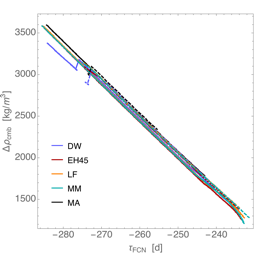
\includegraphics[width=0.50\textwidth]{figures/figa.png}
\label{fig:figa.png}}

\subfloat[]{
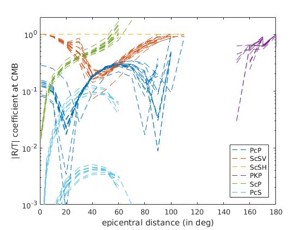
\includegraphics[width=0.50\textwidth]
{figures/figb.png}
\label{fig:figb.png}}

\subfloat[]{
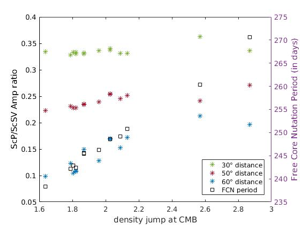
\includegraphics[width=0.50\textwidth]
{figures/figc.png}
\label{fig:figc.png}}
\caption{{a) Relation between density jump at the core-mantle boundary and FCN period for the hot (solid curves) and cold (dashed curves) mantle temperature profile. See Figure 14 and table 4 for legend explanation.
b) Reflexion/transmission coefficients at CMB for various core phases (color code) as a function of epicentral distance (in degrees). The various lines represent the estimates for the 14 a priori models.
c) ScP/ScSV amplitude ratio (stars) and FCN period (in days, open squares) as a function of the relative density jump at the CMB (varying with a priori model). Amplitude ratios are given for 3 different epicentral distance range (color code).}}
\label{fig:figabc}
\end{center}
\end{figure}

\subsubsection{Orbiters/SEIS: Sun k$_2$-ScS travel times}
As noted in Section 2.5, geodesy provides the best constraints on the core size and among those, the Love number k$_2$ is the most sensitive one. For a planet with a liquid core, the elastic deformation of the tide is distributed between the two free surfaces located at the planetary surface on one side and at the Core Mantle Boundary on the other side. A fundamental bias is however found between the shear modulus and the thickness of the mantle, and models with smaller shear modulus but larger mantle will lead to similar k$_2$. See Lognonn\'e \& Johnson (2011, 2015) for an example of this non-unicity of the k$_2$ constraints for the Moon. The 4.9\% error in the $k_2$ determination leave therefore a wide range of freedom in the core size.\\
For ScS travel times, the bias between S waves velocities and mantle depth is the opposite and smaller velocities request smaller depth for a given travel time. The joint inversion of both k$_2$ and ScS travel time will therefore improve greatly the determination of both the mantle structure and depth of the CMB.
Figure \ref{fig:FigureScS.png} shows the differences in core size of the Reference models, detailed in section 3.3 and listed in Table \ref{table:TableModel}. The core radius varies from 1520 km for model SAAK up to 1850 km for model EH45TC. SAAK model, which is has a marked shear waves low velocity zone in the mantle, illustrates well the bias between core depth and mantle shear wave velocity discussed above. If we do not consider such low velocity zone, all models without strong low velocity zone range therefore from 1685km to 1850 km, $\pm$ 82.5 km around the median core radius. As discussed above and already shown by Panning et al. (2017), the core reflected travel time of ScS will provide key new and robust constraints on the core size as illustrated on Earth and more recently on the Moon by Weber et al. (2011) and Garcia et al. (2011). This is also demonstrated by the 150 sec of travel times differences between the two extreme ScS travel times. These two data will therefore be crucial in determining the deep Mars structure and, together with RISE constraints, providing the core radius.
\begin{figure}[h!]
\begin{center}
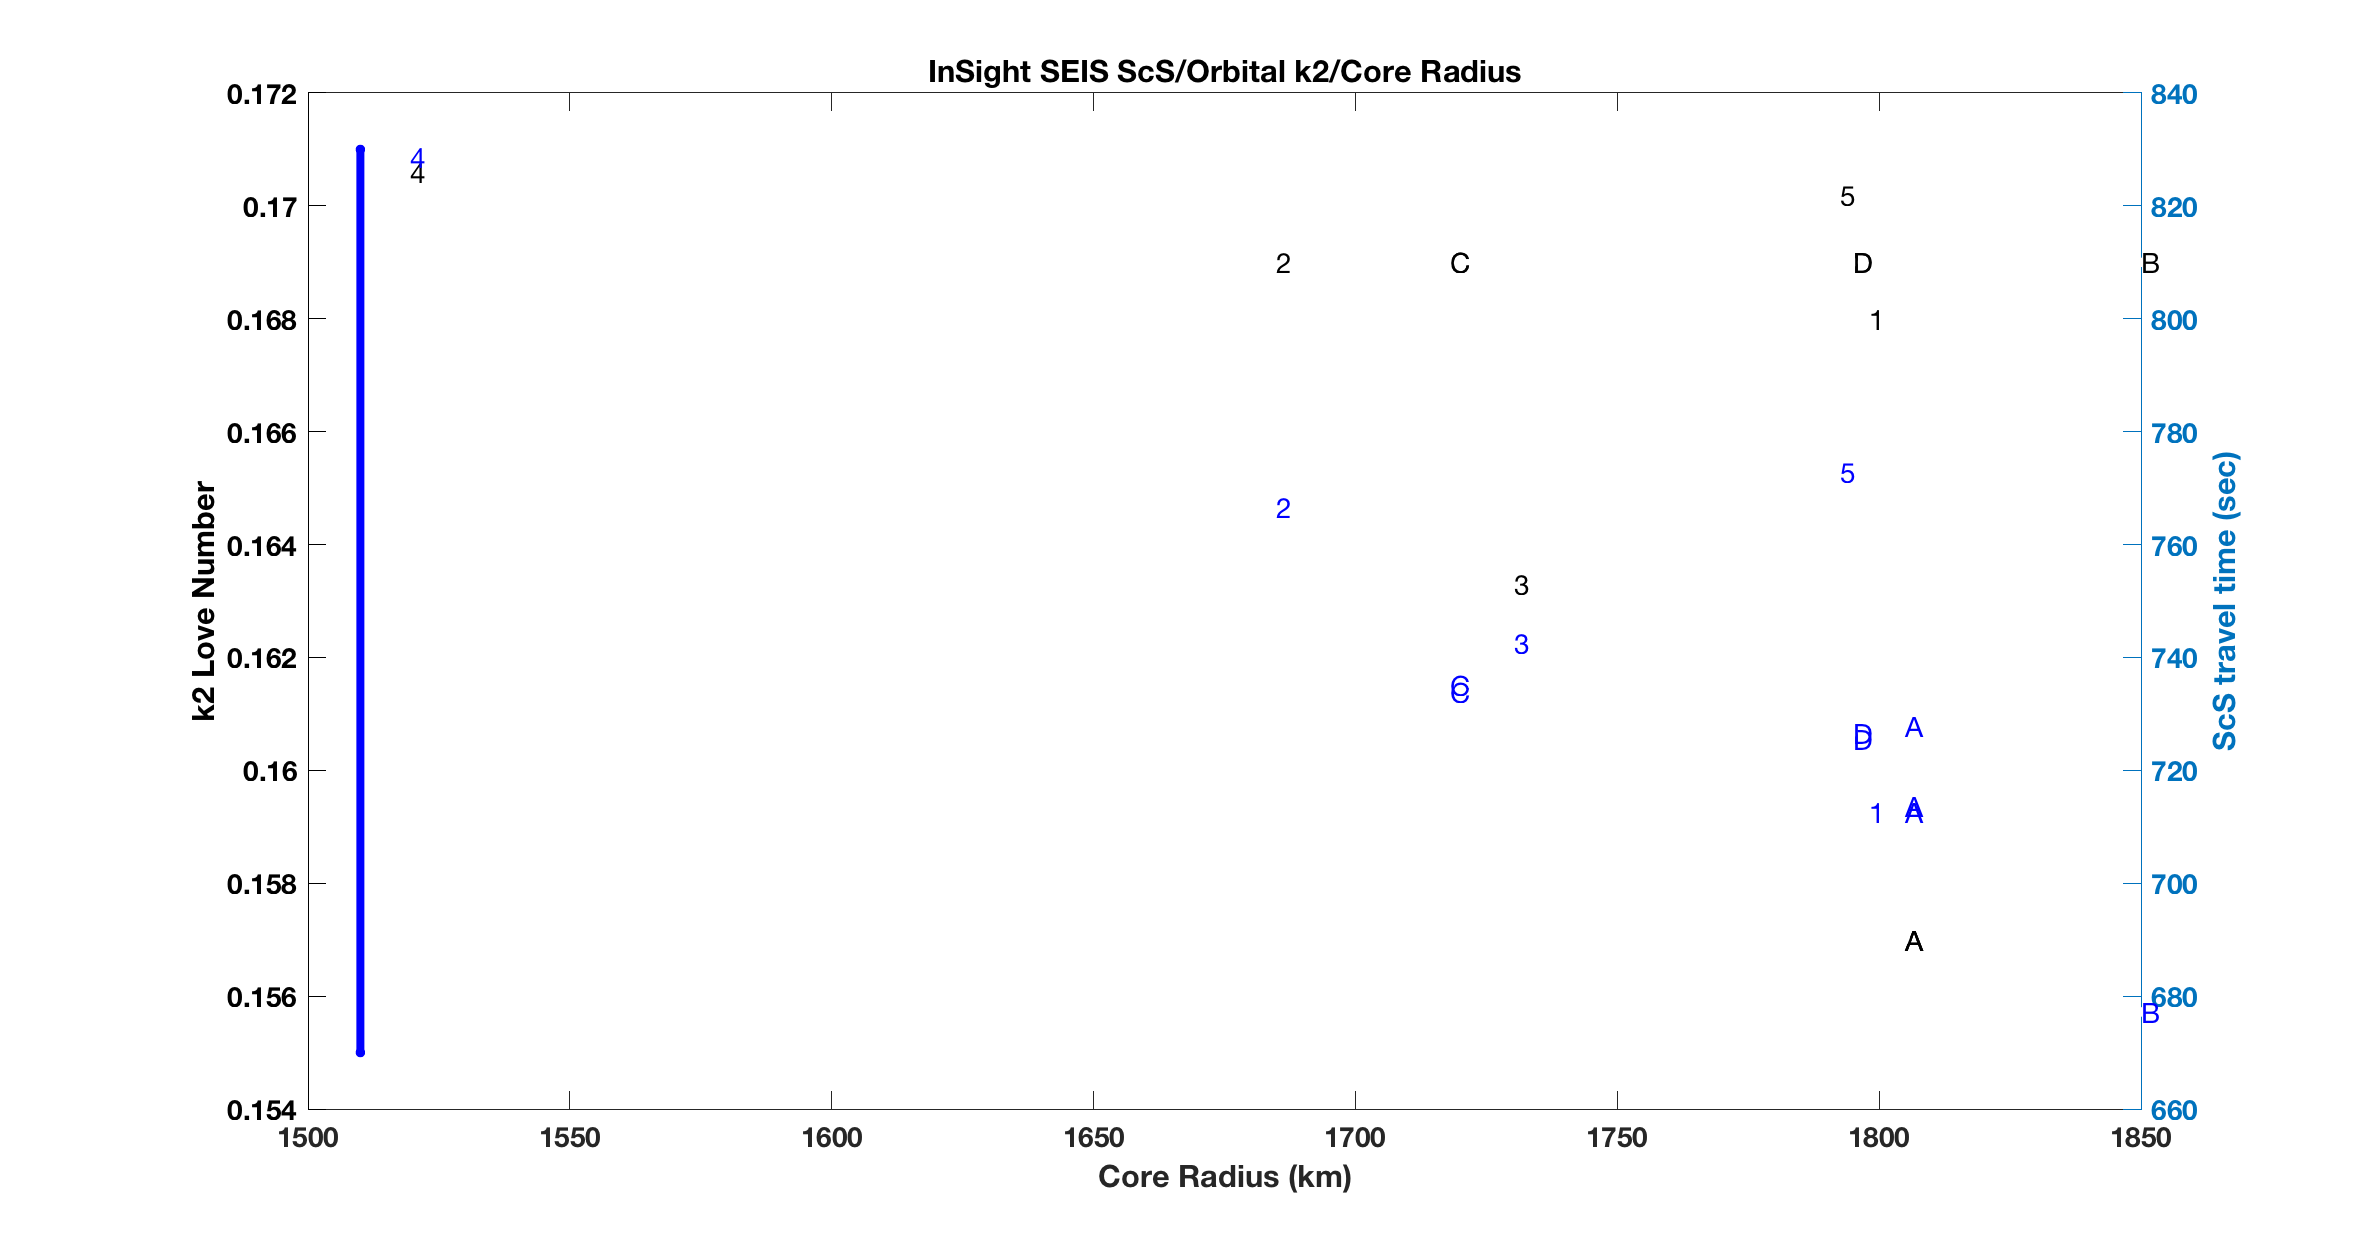
\includegraphics[width=1\textwidth]
{figures/FigureScS.png}
\caption{Values of the Love number k$_2$ (in black on the left) and of the ScS travel time (in blue on the right) for all Reference models described in section 3.3. See Table \ref{table:TableModel} for all values as well as model Letter.}
\label{fig:FigureScS.png} 
\end{center}
\end{figure}

\subsubsection{SEIS/IFG: Vs-Qs and electrical conductivity measurements}

Another important geophysical parameter which can be estimated in advance of the arrival of InSight is the electrical conductivity of the Martian mantle, which represents a signature of the interior which is complementary to seismic velocity (Khan et al., 2006a,b). Such complementarity of magnetic sounding and seismic studies has been demonstrated using Martian synthetic data \citep{Mocquet&Menvielle2000, Verhoeven2005}. The mantle of Mars is characterized by a high iron content \citep{McSween1994}. This result in an order of magnitude increase in the electrical conductivity profile compared to that for the Earth's mantle \citep{Vacher&Verhoeven2007}.

Laboratory measurements of the electrical conductivity of hydrogen-iron bearing mantle silicate minerals have shown that different conduction mechanisms, involving different charge carriers, occur at pressure and temperature conditions relevant to planetary mantles \citep[see e.g. the reviews of][]{Yoshino2010, Karato2011}. In a recent paper, \cite{Verhoeven&Vacher2016} have shown that the small polaron conduction, associated with charge transfer between ferrous and ferric ions, dominates the conductivity at iron and water contents relevant to the Martian mantle.

Figure \ref{fig:conduct.png} shows the electrical conductivity profiles computed using the modeling of \cite{Verhoeven&Vacher2016} for compositions and temperature profiles of the Martian mantle associated with the MSS models of \cite{Panning2016}. The electrical conductivity for the laboratory-based composition model of \cite{Bertka1997}, along with the data-based profile derived by \cite{Civet&Tarits2014} from MGS magnetic field measurements are shown for comparison. In the first thousand km depth, different composition models for the same temperature profile have almost the same electrical conductivity. In contrast, there is a difference of almost one order of magnitude between the electrical conductivity for the cold and hot temperature profiles for a given composition. This suggests that the electrical conductivity can be considered as a good proxy of the mantle temperature in this depth range. This conclusion does not hold below 1000 km depth, where high pressure phases lead to an increasing dependence of electrical conductivity on composition effect. Note that the \cite{Civet&Tarits2014} profile is characterized by 180 km layer thickness which induces some uncertainty in the location of the olivine transition around 1000 km depth.


\begin{figure}[h!]
\begin{center}
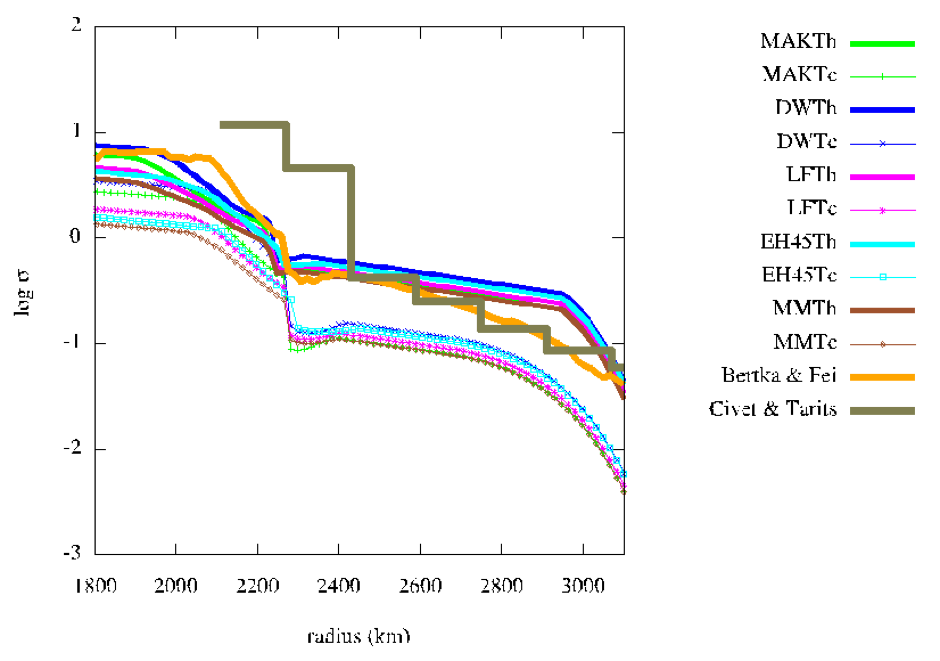
\includegraphics[width=0.75\textwidth]
{figures/Figconduct.png}
\caption{Electrical conductivity profiles corresponding to the composition and temperature profiles associated to the MSS models of Panning et al. (2017) and computed using the modeling of Verhoeven and Vacher (2016). MAK, DW, LF, EH45, MM represent the composition models of Morgan and Anders (1979), Dreibus and W\"{a}nke (1985), Lodders and Fegley (1997), Sanloup et al. (1999) and Mohapatra and Murty (2003), respectively whereas Th and Tc represent end- members temperature profiles from Plesa et al. (2016). The reference models of Bertka and Fei (1997) and Civet and Tarits (2014) are shown for comparison.}
\label{fig:conduct.png} 
\end{center}
\end{figure} 

\subsubsection{Velocity/density jump at the Moho}
Since the Martian surface is characterized by dipole topography, Mohorovicic discontinuity distribution will principally follow the topography anomaly in the opposite-sign manner due to the process of isostatic compensation. A combination of the topography measurement provided by Mars Orbiter Laser Altimeter (MOLA) and the Bouger anomalies estimated from MGS has enabled us to construct the models of Moho depth distributions (e.g. Neumann et al. 2004). The mean crustal thickness is believed to be 50-100 km with 600 kg/m$^3$ of density contrast. However, the ill-posedness of linear inversions hinders an unambiguous determination of crust-mantle density contrast and Mohorovicic depth. Chujkova et al. (2014) proposed to take into account the contribution of the quadratic terms of topographic masses and density contrast in the external gravity potential in order to tackle the problem, showing the feasibility in Earth’s case, but the spherical harmonic degree considered is very low (18). Furthermore, Mohorovicic estimation using potential data is hampered by a strong non-equilibrium due to the dichotomy (e.g. Gudkova et al. 2017) and the sharpness and lateral distribution of density around Moho discontinuity are really hard to look at. It is thus important to give a seismic constraint on seismic velocity and density jump and their depths from SEIS measurement. Since the velocity-density empirical relationship (e.g. Barton 1986) could sometimes encounter disagreements even in some places in Earth (e.g. Hsieh \& Yen 2016), it will be interesting to first investigate velocity by teleseismic refraction data independently from potential data, so that we be able to infer rock types.

Yet, seismological observations from refraction data might not be sufficient to constrain the Mohorovicic discontinuity due to its smoothed feature. In order to exploit the information on the structural effects beneath the seismic station embedded especially in high-frequency contents of SEIS teleseismic events, we will calculate receiver functions by removing the source-time function effects as well as the far deep mantle structure (e.g. Vinnik 1977; Kumar et al. 2010) and we will be also able to perform multi-parameter inversion using the receiver function (e.g. Bodin et al. 2014). Fig. 18 shows receiver functions for several given models with various epicentral distances.

\begin{figure}[h!]
\begin{center}
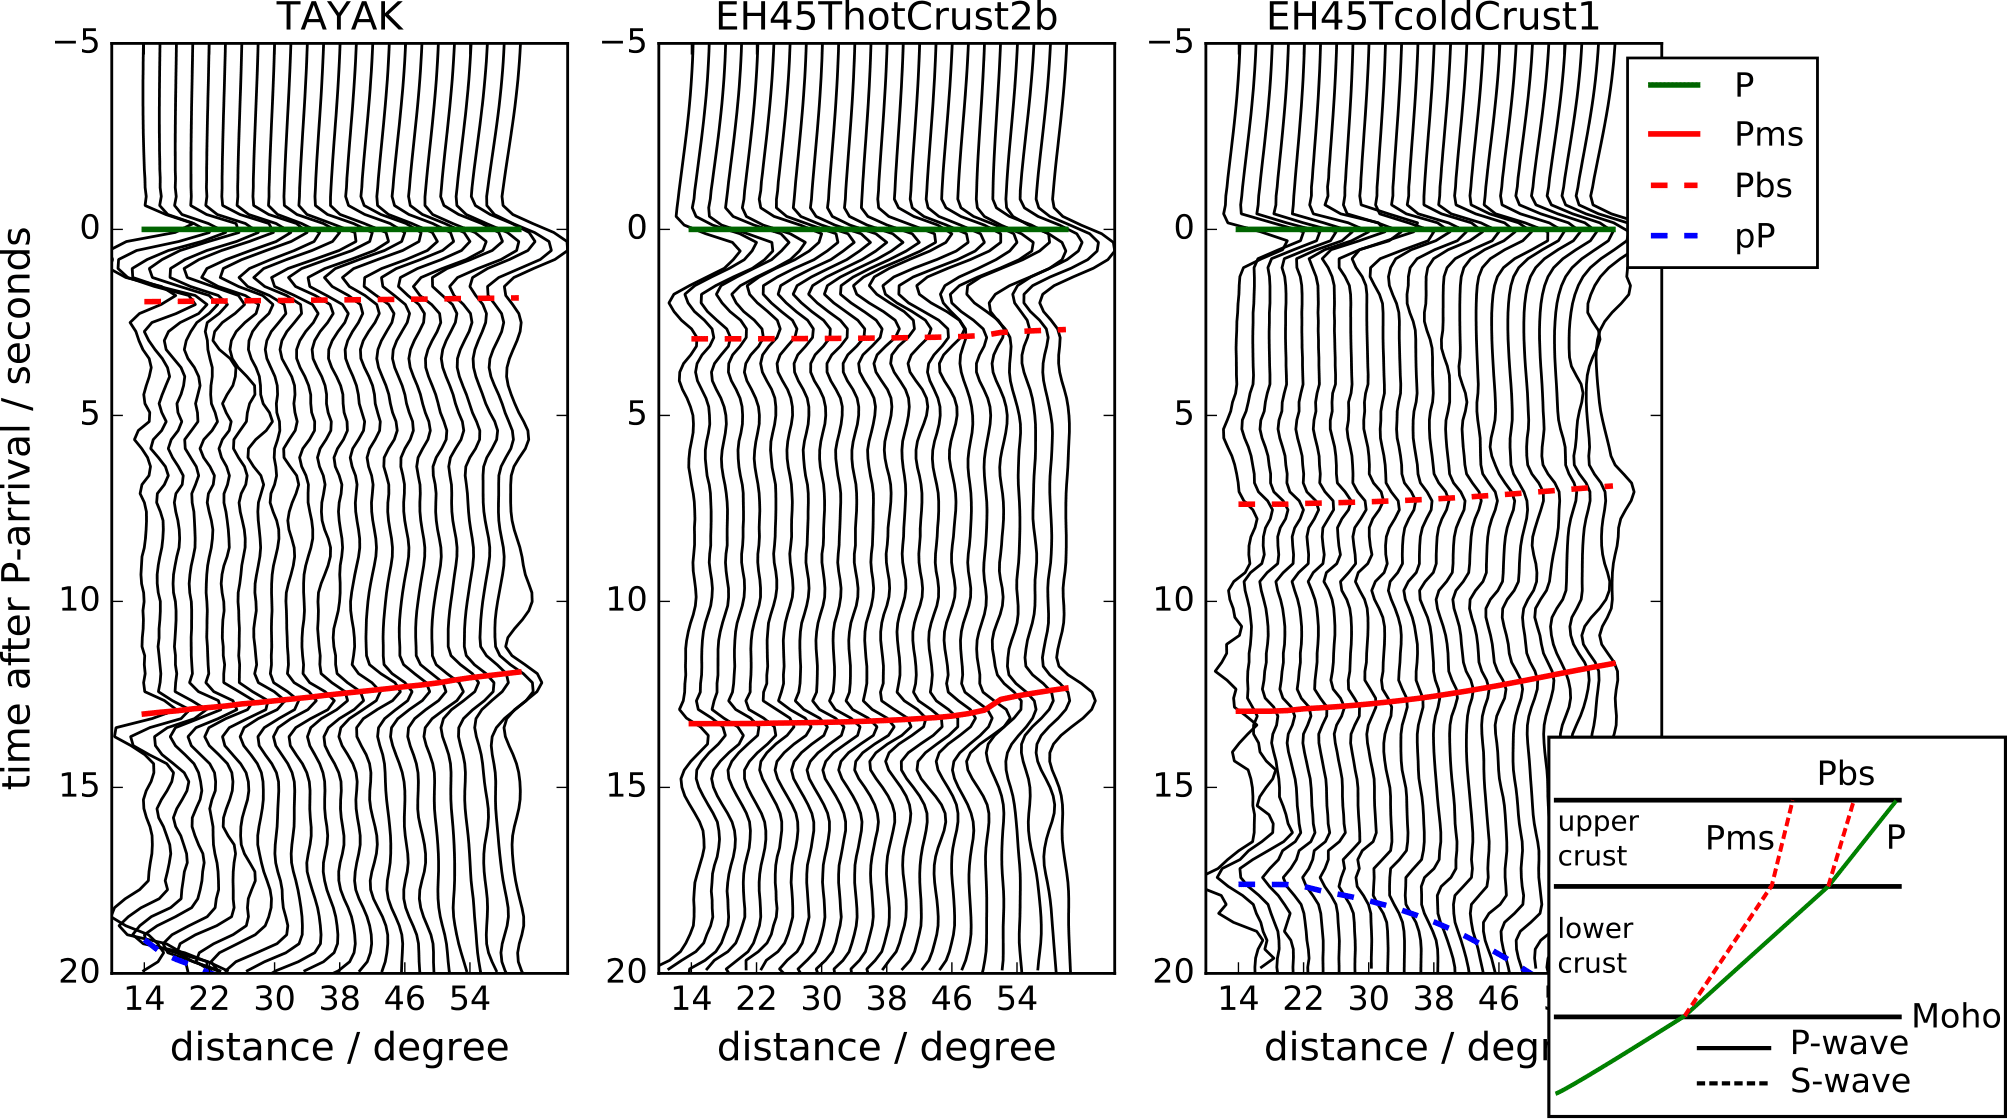
\includegraphics[width=1.0\textwidth]
{figures/Fig_waveforms.png}
\caption{Receiver function example for three models of the InSight Blindtestmodel suite \citep{Clinton2017}. The waveforms show the R-component of the P-wave coda of a 60 km deep event in various distances. Highlighted are the theoretical arrival times of P-S conversions at the Moho (Pms) or a mid-crust-discontinuity (Pbs). The converted waveforms are relatively low in amplitude, but especially Pms is clearly visible. The waveforms were calculated using AxiSEM and Instaseis \citep{Nissen-Meyer2014, VanDriel2015}}
\label{fig:waveform.png} 
\end{center}
\end{figure} 


Another factor to be considered is the existence/absence of an upper mantle low velocity zone due to a thick stagnant lid or local dissipation in the Martian mantle (Zheng et al. 2015), that can provoke a shadow zone for direct P- and S-waves. It will result in difficulty of receiver function analysis described above, although long-wavelength 1D imaging will not really affected by its existence or absence (e.g. Khan et al. 2016).


